\subsection{Background segmentation}

The background segmentation node is based on the backgroundSubtractorMOG2 from OpenCV \cite{BGS} which uses Gaussian mixtures to perform the segmentation. The background segmentation results in a binary image of the foreground. 

\begin{figure}[H]
\begin{center}
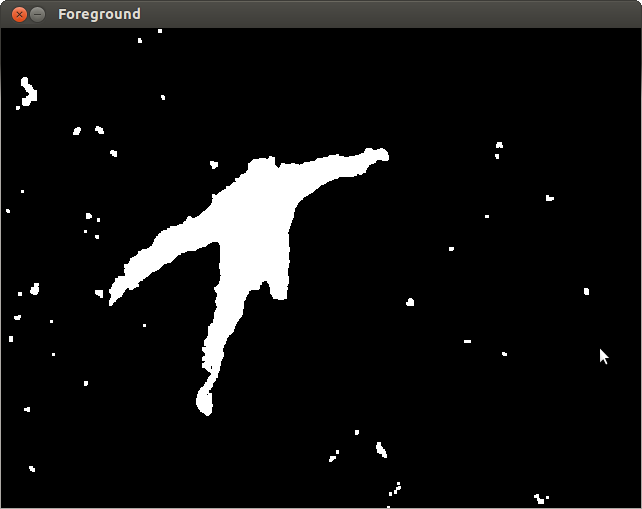
\includegraphics[width=12 cm]{screenshot_foreground_image}
\caption{Foreground from background segmentation}

\end{center}
\end{figure}

The foreground and depth image are used to construct a point cloud. For each foreground pixel the corresponding depth value $P_z$, pixel coordinates $P_x$, $P_y$ and intrinsic parameter can be used to obtain the world coordinates as follows.

$P_x = (p_x - c_x) * P_z / f_x$
$P_y = (p_y - c_y) * P_z / f_y$

and the point $P = [P_x, P_y, P_Z]^T$

By applying these formulas to all foreground pixels the point cloud is achieved.


